\documentclass[10pt,preprint]{sigplanconf}
\usepackage[utf8]{inputenc}
\usepackage{graphicx}
\usepackage{fancyhdr}
\usepackage{amsmath}
\usepackage{xfrac}
\usepackage{listings}
\usepackage{tikz}
\usetikzlibrary{trees,automata,positioning,arrows}
\usepackage[sc]{mathpazo}
\usepackage{titlesec}
\usepackage{etoolbox}
\usepackage{amsthm,amssymb}
\usepackage{array}
\usepackage{mathtools}
\usepackage{bussproofs}
\usepackage[numbers]{natbib}
\DeclarePairedDelimiter{\ceil}{\lceil}{\rceil}

\newcommand{\mytitle}{Timing-sensitive Secure Multi-Execution}
\authorinfo{Christopher Schuster}
           {University of California, Santa Cruz}
           {\texttt{\{cschuste\}@ucsc.edu}}


\title{\mytitle}
% \pagestyle{fancy}
% \fancyhf{}
% \titleformat{\section}{\normalfont\Large\bfseries}{}{0em}{}
% \titleformat{\subsection}{\normalfont\bfseries}{}{0em}{}
% \renewcommand{\thesection}{\arabic{section}}
% \renewcommand{\thesubsection}{\arabic{section}.\alph{subsection})}
\tikzstyle{t} = [circle, draw=black, thick, fill=none, text centered, minimum height=8mm,minimum width=8mm]
\tikzstyle{level 1}=[level distance=1.5cm, sibling distance=2cm]
\tikzstyle{level 2}=[level distance=1.5cm, sibling distance=1cm]
\tikzstyle{level 3}=[level distance=1.5cm, sibling distance=1cm]
\tikzstyle{level 4}=[level distance=1.5cm, sibling distance=1cm]
% \lhead{\myauthor}
% \rhead{\mytitle}
% \cfoot{\thepage}
% \newcommand{\zerodisplayskips}{%
%   \setlength{\abovedisplayskip}{0pt}
%   \setlength{\belowdisplayskip}{0pt}
%   \setlength{\abovedisplayshortskip}{0pt}
%   \setlength{\belowdisplayshortskip}{0pt}}
% \appto{\normalsize}{\zerodisplayskips}
% \appto{\small}{\zerodisplayskips}
% \appto{\footnotesize}{\zerodisplayskips}
\lstdefinelanguage{JavaScript}{
  keywords={typeof, new, true, false, catch, function, return, null, catch, switch, var, if, in, while, do, else, case, break, fx},
  keywordstyle=\color{darkgray}\bfseries,
  ndkeywords={class, export, boolean, throw, implements, import, this},
  ndkeywordstyle=\color{darkgray}\bfseries,
  identifierstyle=\color{black},
  sensitive=false,
  comment=[l]{//},
  morecomment=[s]{/*}{*/},
  commentstyle=\color{purple}\ttfamily,
  stringstyle=\color{gray}\ttfamily,
  morestring=[b]',
  morestring=[b]"
}

\lstset{language=JavaScript,
        basicstyle=\ttfamily,
        aboveskip={0.5\baselineskip},
        belowskip={0.5\baselineskip},
        showstringspaces=false,
        frame=t,
        captionpos=b}
% Don't indent paragraphs.
% \setlength{\parindent}{0em}
% \setlength{\parskip}{0.5\baselineskip}
% \newcommand{\prob}[1]{\setcounter{section}{#1} \addtocounter{section}{-1} \section{} }
\newcommand{\lab}[1]{\RightLabel{\textsc{\small #1}}}
\newcommand{\ov}[2]{\genfrac{}{}{0pt}{}{\text{\textbf{#1}}}{\text{\footnotesize{#2}}}}
\newcommand{\arrayStretch}{1.28}

\renewcommand{\t}[1]{~\text{#1}~}
\newenvironment{bpt}{\leavevmode\hbox\bgroup}{\DisplayProof\egroup}

\newtheoremstyle{plain}{\topsep}{\topsep}{\itshape}{}{\scshape}{.}{5pt plus 1pt minus 1pt}{}
\newtheorem{theorem}{Theorem}
\newtheorem{lemma}{Lemma}
\newtheorem{definition}{Definition}

\begin{document}
\maketitle

\abstract{
By using an information flow policy, information from annotated sources cannot be leaked to unauthorized observers even in the presence of programming errors.  While explicit and implicit leaks can be prevented with labeled data, secure multi execution and static approaches, closing the timing covert channel on a shared processor requires a customized secure scheduler.  This paper introduces dynamic information flow control based on secure multi-execution of a small lambda calculus with labeled channels and presents two different secure scheduling strategies: a simple and inefficient round robing scheduling between known labels, and more sophisticated scheduling for dynamic labels.
}

\section{Introduction}

Secure information flow ensures that private information can never leak to or indirectly influence public/unauthorized recipients.  However, if the program performs both private and non-private computation on the same machine, an external observer might learn about non-private data through the timing of the execution which might be affected by other (private) executions running on the same machine.

As an example, the following NodeJS JavaScript web server has an internal ``private'' request counter which gets incremented at every request and logged to a local console by repeatedly printing a dot.  If every \verb+console.log+ operation takes roughly the same time, then the time it takes to fully complete a request scales linearly with the private counter.  The time of the private part of the execution therefore has to be hidden from the public observer.

\subsection{Secure multi execution}

Secure multi-execution as introduced by Devriese et al. \cite{devriese2010} protects against both direct and indirect information leaks by executing the program once for each security level, e.g. H(igh) and L(ow).  Each execution can only write information to channels on the exact same level (other writes will be suppressed) and read from channels that have the same or a lower level than the execution (reads from a higher level return a default value).

For the example in Listing \ref{lst:express}, secure multi execution could ensure that the private information in the \verb+counter+ variable cannot influence public observable output.  The \emph{public} thread of execution reads a default value for the counter, e.g. 0, and suppresses the update and the \verb+console.log+ call while the \emph{private} thread of execution skips the \emph{res.send} call.

\begin{lstlisting}[float,label=lst:express,caption={JavaScript Server Code which leaks the value of the private request counter via the timing covert channel.}]
var app = require('express')();
var counter = 0;   // Private counter

app.post('/', function (req, res) {
  counter++;
  for (var i = 0; i < counter; i++) {
    console.log('.');
  }
  res.send('Request counted.');
});

var server = app.listen(3000);
\end{lstlisting}

\subsection{Timing covert channels}

Despite information flow control through secure multi execution, the code shown in Listing \ref{lst:express} is still vulnerable to attacks through the timing covert channel.  We have to assume that an attacker would be able to send HTTP requests and externally measure the time between request and response.  Therefore, this time should not depend on the time for logging the secret value of the counter, as mentioned above.

In order to close this timing covert channel, the private and public execution threads need to be disentangled and scheduled in a way that prevents an attacker from learning about other concurrently executing threads.

Kashyap et. al.~\cite{kashyap2011} previously explored different scheduling strategies for termination and timing-sensitive secure multi execution.  A na\"ive scheduling strategy would always prioritize public execution over private execution and thereby hide concurrent private execution, which may depend on private data, from public execution with its externally observable timing.  However, this might cause private execution threats to starve and it does not work if there are more security levels than just private and public.

\begin{figure}
\begin{center}\vspace{-2ex}
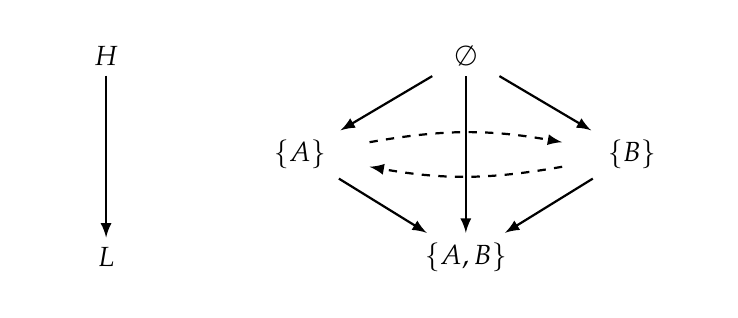
\begin{tikzpicture}
\tikzstyle{c} = [minimum width=5em]
\tikzstyle{d} = [rectangle, draw, thick, minimum height=6.5mm,minimum width=5em]
\matrix[column sep=1em,row sep=2em]
{
  \node[c] (h) {$H$}; & & & \node[c] (ab) {$\emptyset$}; & \\
                      & & \node[c] (a) {$\{A\}$}; & & \node[c] (b) {$\{B\}$}; \\
  \node[c] (l) {$L$}; & & & \node[c] (n) {$\{A,B\}$}; & \\
};
\draw[-latex, thick] (h) -- (l);
\draw[-latex, thick] (ab) -- (a);
\draw[-latex, thick] (ab) -- (b);
\draw[-latex, thick] (a) -- (n);
\draw[-latex, thick] (b) -- (n);
\draw[-latex, thick] (ab) -- (n);
\draw[-latex, thick, dashed] (a) to [bend left=10] (b);
\draw[-latex, thick, dashed] (b) to [bend left=10] (a);
\end{tikzpicture}
\end{center}
\caption{In contrast to binary security levels $H$ and $L$, levels in a more complex security lattice might not have a total order.  }
\label{fig:lattice}
\end{figure}

As an example, Figure \ref{fig:lattice} shows two different designs of possible security levels, the simple public/private binary system, and a more complex lattice with additional two principals $A$ and $B$ who can designate information as private for each individually.  Here, $\{ A,B \}$, the public security level of information that both $A$ and $B$ can access, might influence other security levels but should not be influenced by information private to either $A$ or $B$.  The two security levels $A$ and $B$, on the other hand, are incomparable.  For SME, this means that execution that is private for $A$ and execution that is private for $B$ have to be hidden from each other with no difference in scheduling priority.  Furthermore, the maximum execution time available to each incomparable security level cannot be influenced by timing and termination of other incomparable security levels.

\section{Explicit, streaming I/O}

Consider a programming language based on lambda calculus with simple IO as shown in Figure \ref{fig:io}.  Part of the execution environment is a set of buffers $\vec{n}$ for each channel name $n_c$.

\begin{figure}
\[ \arraycolsep=1.6pt\def\arraystretch{1.5}
\begin{array}{rl}
  \multicolumn{2}{l}{x : \t{Identifier}~\hfill~n : \t{Literal}~\hfill~B : n \mapsto \vec{n} ~\t{(Buffers)}} \\[1ex]
  e := & v ~|~ x ~|~ e ~ e ~|~ e ; e ~| \t{read} e ~| \t{write} e~e\\
  v := & n ~|~ \lambda x.~e \\[1ex]
  E[\circ] := & \circ ~|~E~e~|~v~E~|~E~;~e~|~v~;~E \\
              & ~~~ | \t{read} E~| \t{write} E~e | \t{write} v~E \\[1ex]
  \multicolumn{2}{c}{recv : n \mapsto () + \vec{n} ~~~~ \rightarrow : B,e \times B,e}
  \end{array}
\]
\begin{center}
\begin{bpt}
  \AxiomC{$B, e~\fCenter{\ \rightarrow\ }~B', e' $}
  \lab{e-ctx}
  \UnaryInfC{$B, E[e] \fCenter{\ \rightarrow\ } B', E[e'] $}
\end{bpt}
\begin{bpt}
  \AxiomC{${~}^{~}_{~}$}
  \lab{e-seq}
  \UnaryInfC{$B, v_1;v_2 \rightarrow B, v_2 $}
\end{bpt} \\[1em]
\begin{bpt}
  \AxiomC{}
  \lab{e-app}
  \UnaryInfC{$B, (\lambda x. e)~v~\rightarrow~B, e[x \mapsto v] $}
\end{bpt} \\[1em]
\begin{bpt}
  \AxiomC{$B(n_c) = (n_0,n_1, ...)$}
  \lab{e-read}
  \UnaryInfC{$B, \t{read} n_c~\rightarrow~B[n_c \mapsto (n_1,...)], n_0 $}
\end{bpt} \\[1em]
\begin{bpt}
  \AxiomC{$B(n_c) = (...~, n_k)$}
  \lab{e-write}
  \UnaryInfC{$B, \t{write} n_c~n~\rightarrow~B[n_c \mapsto (...~,n_k, n)], n_c $}
\end{bpt} \\[1ex]

\end{center}
\caption{Operational semantics of a simple language with buffered, streaming I/O operations.}
\label{fig:io}
\end{figure}

The formalism is underspecified in the sense that buffer may also be modified by the environment which is not modeled.  Otherwise, every value in a buffer is the result of a write operation in a FIFO way.  When reading inputs, the evaluation can only step if there are available values in the buffer, otherwise it will block until the environment changes (or other concurrent threads) provide a value in the buffer.  The buffer itself is inconsequential for simply performing IO but becomes important for secure multi execution.

\subsection{Secure multi execution}

Given a fixed set of security labels $\mathcal{L}$, secure multi execution involves evaluating the program once for each label $l$.  The extended formalism and operational semantics based on the lambda calculus in Figure \ref{fig:io} is shown in Figure \ref{fig:io-sme}.

It is noteworthy that every label has its own read buffer.  Values from the environment, or written by other threads, will be added to the buffer of all labels.  This ensures that secure multi executions reuses previously read values.  Additionally, reads will return a default value (or alternatively some error value $\bot$) if values from a read labeled $l_c$ are not allowed to flow to the currently execution label $l$, and writes will be suppressed if the denoted write level differs from the executing label.  This prevents leaks from higher information to lower channel and it also cancels duplicated output due to secure multi execution.

Additionally, there are now two different evaluation relations.  The single thread evaluation $\rightarrow_l$ performs one step of evaluation of $e$ with channels $C$ under the label $l$.  The overall evaluation $\leadsto$ has channels $C$, one program/term per label $\Sigma$ and a list of labels $\vec{l}$.

\begin{figure}
\[ \arraycolsep=1.6pt\def\arraystretch{1.5}
\begin{array}{rl}
  \multicolumn{2}{c}{l \in \mathcal{L} : \t{Labels}~\hfill~B : l \times n \mapsto \vec{n} ~\t{(Buffers)}} \\
    e := & ... ~| \t{read} l~e ~| \t{write} l~e~e\\
    E[\circ] := & ...~| \t{read} l~E~| \t{write} l~E~e | \t{write} l~v~E\\
\multicolumn{2}{l}{
\rightarrow_l : B,e \times B,e~\hfill~\leadsto : B, \Sigma, \vec{l} \times B, \Sigma, \vec{l}~\hfill~
\Sigma : l \mapsto e}
  \end{array} \\
\]

\begin{center}
  (\textsc{e-ctx}, \textsc{e-app} and \textsc{e-seq} for $\rightarrow_l$ as in Figure \ref{fig:io}) \\[1em]

\begin{bpt}
  \AxiomC{$l_c \not \sqsubseteq l$}
  \lab{e-read-default}
  \UnaryInfC{$B, \t{read} l_c~n_c~\rightarrow_l~B, n_{default} $}
\end{bpt} \\[1em]
\begin{bpt}
  \AxiomC{$l_c \sqsubseteq l$}
  \AxiomC{$B(l, n_c) = (n_0, n_1, ...)$}
  \lab{e-read}
  \BinaryInfC{$B, \t{read} l_c~n_c \rightarrow_l B[(l, n_c) \mapsto (n_1,...)], n_0 $}
\end{bpt} \\[1em]
\begin{bpt}
  \AxiomC{$l \not = l_c$}
  \lab{e-write-suppress}
  \UnaryInfC{$B, \t{write} l_c~n_c~n_o~\rightarrow_l~B, n_c $}
\end{bpt} \\[1em]
\begin{bpt}
  \alwaysNoLine
  \AxiomC{$l = l_c$}
  \UnaryInfC{$B' = B[(l', n_c) \mapsto B(l',n_c) \cdot n_0~|~l \sqsubseteq l' \in \mathcal{L}]$}
  \alwaysSingleLine
  \lab{e-write}
  \UnaryInfC{$B, \t{write} l_c~n_c~n~\rightarrow_l~B', n_c $}
\end{bpt} \\[1em]
\begin{bpt}
  \AxiomC{$\Sigma(l) = e$}
  \AxiomC{$B, e \rightarrow_l B', e'$}
  \lab{s-step}
  \BinaryInfC{$B, \Sigma, (l, l', ...) \leadsto B', \Sigma[l \mapsto e'], (l', ...~, l) $}
\end{bpt} \\[1em]
\begin{bpt}
  \AxiomC{$\Sigma(l) = e$}
  \AxiomC{$B, e \not \rightarrow_l$}
  \lab{s-idle}
  \BinaryInfC{$B, \Sigma, (l, l', ...) \leadsto B, \Sigma, (l', ...~, l) $}
\end{bpt}

\end{center}
\caption{Secure Multi Execution with explicitly labeled IO and round-robin scheduling based on the language in Figure \ref{fig:io}.}
\label{fig:io-sme}
\end{figure}

Given a program $e$ and a set of security labels $\mathcal{L}$, the initial state of the overall computation $\leadsto$ is denoted by $B = \emptyset$, $\Sigma = [e \mapsto l ~|~ l \in \mathcal{L}]$, $\vec{l} = \sigma(\mathcal{L})$ where $\sigma(\mathcal{L})$ is an arbitrary permutation of security labels $l$.

At each step $\leadsto$ the scheduling order $\vec{l}$ will be rotated which corresponds to a simple round robin scheduling.  However, terminated and blocked threads will still be scheduled by the rule \textsc{s-idle} which forces the execution to wait the exact same amount of time that \textsc{s-step} takes for executing a single execution step $\rightarrow_l$.  Alternatively, \textsc{s-step} might run for each a fixed budget of $n$ steps which also involves waiting $n-k$ steps if the threads blocks or terminates after $k$ steps.

\subsection{Non-interference}

With SME, only threads running with label $l$ can produce output to $l$-labeled channels.  Therefore, it is sufficient to prove that a thread running with label $l$ cannot be influenced by any information labeled $l' \not \sqsubseteq l$ to prove that the resulting system prevents leaks of information to unauthorized channels.

To prove this kind of non-interference, we define an equivalence  $\approx_l$ of execution configurations $B,\Sigma,\vec{l}$ which only differ in information unauthorized for $l$.  In contrast to other dynamic information flow strategies, each thread in secure multi execution operates on its own program which never includes unauthorized sub-programs.  Additionally, we restrict buffers in a way that buffers accessible to $l$ include no information private to $l$ and the scheduling order $\vec{l}$ is assumed to be public.
\[ B_1,\Sigma_1, \vec{l} \approx_l B_2,\Sigma_2, \vec{l}~\hat{=}~ \epsilon_l(\Sigma_1) = \epsilon_l(\Sigma_2) \wedge \epsilon_l(B_1) = \epsilon_l(B_2) \]

Here, the erasure function $\epsilon_{l}$ removes higher-level threads and buffers from $\Sigma$ and $B$ which are not allowed to flow into $l$:
\[\arraycolsep=1.6pt\def\arraystretch{\arrayStretch}
\begin{array}{lr}
  \epsilon_{l}(\Sigma) = [ l_e \mapsto \Sigma(l_e) ~|~ l_e \in dom(\Sigma) \wedge l_e \sqsubseteq l ] \\
  \epsilon_{l}(B) = [ (l_c, n_c) \mapsto B(l_c, n_c) ~|~ (l_c, n_c) \in dom(B) \wedge l_c \sqsubseteq l ]
\end{array} \]

As a first step, we need to show that a single step of execution for two $l$-equivalent configurations cannot depend on information above $l$.

\begin{theorem}[Termination-sensitive non-interference]
  For all labels $l$, $l_e \in \mathcal{L}$, and $l$-equivalent configurations $B_1,e_1 \approx_l B_2,e_2$, a step of execution $\leadsto$ should preserve $l$-equivalence.
  \begin{align*}
    B_1,\Sigma_1, \vec{l_1} \leadsto B'_1,\Sigma'_1, \vec{l'_1} ~\wedge~B_2,\Sigma_2,\vec{l_2} \leadsto B'_2,\Sigma'_2, \vec{l'_2} \\
    \Rightarrow B'_1,\Sigma'_1, \vec{l'_1} \approx_l B'_2,\Sigma'_2, \vec{l'_2}
  \end{align*}
\end{theorem}

\begin{proof}
  Assuming $B_1,\Sigma_1, \vec{l_1} \approx_l B_2,\Sigma_2, \vec{l_2}$, it follows that
  \[ \epsilon_l(B_1) = \epsilon_l(B_2)~\wedge~\epsilon_l(\Sigma_1) = \epsilon_l(\Sigma_2) ~\wedge~ \vec{l_1} = \vec{l_2}\]
  with the same scheduled label $l_e$.
  \[ \vec{l_1} = (l_e, ...) = \vec{l_2} \]

  For arbitrary labels $l$ and $l_e$, we can distinguish two different cases:

  \textbf{(Case 1: $l_e \not \sqsubseteq l$)}
  
  \noindent A step $\leadsto$ by an arbitrary configuration $B,\Sigma$ uses either the rule \textsc{s-step} or \textsc{s-idle}.

  (Case 1.a \textsc{s-idle}) In this case, the configuration did not change except for a rotation of schedule $\vec{l}$.  In particular, $B = B' ~\wedge~ \Sigma = \Sigma'$, which implies
  \[ B,\Sigma, \vec{l'} \approx_l B', \Sigma', \vec{l'} \]

  (Case 1.b \textsc{s-step}) Regarding the executing threads $\Sigma$, a step of evaluation with \textsc{s-step} only updates the program of the corresponding label $l_e$.
\[ \Sigma' = \Sigma[l_e \mapsto e'] \]

If $l_e$ is a higher than $l$, execution $\rightarrow_{l_e}$ manipulates a subprogram $\Sigma(l_e)$ which is not part of $\epsilon_l(\Sigma)$, so
\begin{align*}
  & \epsilon_l(\Sigma') = \epsilon_l(\Sigma[l_e \mapsto e']) = \epsilon_l(\Sigma) & (l_e \not \sqsubseteq l)
\end{align*}

Regarding the buffers $B$, a step of evaluation with \textsc{s-step} only changes buffers with the \textsc{e-read} and the \textsc{e-write} rule.

The \textsc{e-read} rule only manipulates a buffer $B(l_e,n_c)$ which is not part of $\epsilon_l(B)$, so
\begin{align*}
  & \epsilon_l(B') = \epsilon_l(B[(l_e,n_c) \mapsto ...]) = \epsilon_l(B) & (l_e \not \sqsubseteq l)
\end{align*}

Additionally, the \textsc{e-write} rule only manipulates buffers $B(l',n_c)$ with $l_e \sqsubseteq l'$.
\begin{align*}
 ~&~ l' \sqsupseteq l_e \not \sqsubseteq l~~\Rightarrow~~l' \sqsupseteq l_e \sqsupset l ~~
  \Rightarrow~~ l' \sqsupset l&\Rightarrow~ l' \not \sqsubseteq l \\
\Rightarrow~&~ \epsilon_l(B') = \epsilon_l(B[l' \mapsto ...]) = \epsilon_l(B) & (l' \not \sqsubseteq l)
\end{align*}

Both of these cases work for both configurations $B_1, \Sigma_1$ and $B_2, \Sigma_2$ and the updated schedule $\vec{l'}$ will always be rotated by one independent of whether \textsc{s-idle} or \textsc{s-step} was used in each case.
\[\arraycolsep=1.6pt\def\arraystretch{\arrayStretch}
\begin{array}{c}
  \epsilon_l(B'_1) = \epsilon_l(B_1) = \epsilon_l(B_2) = \epsilon_l(B'_2)\\
  \wedge~\epsilon_l(\Sigma'_1) = \epsilon_l(\Sigma_1) = \epsilon_l(\Sigma_2) = \epsilon_l(\Sigma'_2) ~\wedge~\vec{l'_1} = \vec{l'_2} \\
  \Rightarrow~B'_1,\Sigma'_1, \vec{l'_1} \approx_l B'_2,\Sigma'_2, \vec{l'_2}
\end{array} \]

\textbf{(Case 2: $l_e \sqsubseteq l$)} If the execution operates on level $l_e \sqsubseteq l$, the scheduled program $e$ will be identical for both $\Sigma_1$ and $\Sigma_2$ due to $l$-equivalence $\Sigma_1 \approx_l \Sigma_2$:
\[ \epsilon_l(\Sigma_1)(l_e) = \Sigma_1(l_e) = e = \Sigma_2(l_e) = \epsilon_l(\Sigma_2)(l_e) \]

A step $\leadsto$ by configuration $B_1,\Sigma_1$ uses either the rule \textsc{s-step} or \textsc{s-idle}.

(Case 2.a \textsc{s-idle}) In this case, we know that $e$ with buffers $B_1$ was not able to step: $B_1,e \not \rightarrow_{l_e}$.

  There are two possible reasons for not stepping.  Either the program terminated, i.e. $e=v$ which implies that the configuration $B_2,e$ cannot step either; or $e$ is a blocking read $e = E[\text{read}~l_c~n_c]$ with buffer $B_1(l_e, n_c) = ()$.  Due to $l$-equivalence, the same has to be true for $B_2$:
  \[ B_1(l_e,n_c) = \epsilon_l(B_1)(l_e,n_c) = \epsilon_l(B_2)(l_e,n_c) = B_2(l_e,n_c) \]

  Since both configurations used rule \textsc{s-idle}, the configurations did not change except for a rotation of schedule $\vec{l}$.
\[\arraycolsep=1.6pt\def\arraystretch{\arrayStretch}
\begin{array}{c}
  B_1 = B'_1 ~\wedge~ \Sigma_1 = \Sigma'_1~\wedge~B_2 = B'_2 ~\wedge~ \Sigma_2 = \Sigma'_2 \\
  \Rightarrow \epsilon_l(B'_1) = \epsilon_l(B_1) = \epsilon_l(B_2) = \epsilon_l(B'_2)\\
  \wedge~\epsilon_l(\Sigma'_1) = \epsilon_l(\Sigma_1) = \epsilon_l(\Sigma_2) = \epsilon_l(\Sigma'_2) ~\wedge~\vec{l'_1} = \vec{l'_2} \\
  \Rightarrow~B'_1,\Sigma'_1, \vec{l'_1} \approx_l B'_2,\Sigma'_2, \vec{l'_2}
\end{array} \]

(Case 2.b \textsc{s-step}) The evaluation rules are non-overlapping except for two possible pairs:
  \begin{itemize}
\item (Rules \textsc{e-read} and \textsc{e-read-default}) For the term ``read $l_c~n_c$'', the label $l_c$ is part of $e$ and will be the same in both $\Sigma_1$ and $\Sigma_2$, so $\l_c \sqsubseteq l$ will evaluate identically for both configurations regardless of buffers.
\item (Rules \textsc{e-write} and \textsc{e-read-write}) Similarly, for the term ``write $l_c~n_c~n$'', the label $l_c$ is part of the program $e$, so $\l \sqsubseteq l_c$ will evaluate identically for both configurations.
  \end{itemize}

  As the step taken by $\rightarrow_l$ is unique for $e$ and $l$, the two configurations $B_1,e$ and $B_2,e$ have to use the same rule.

  In case the configurations steps with either \textsc{e-app}, \textsc{e-seq}, \textsc{e-read-default} or \textsc{e-write-suppress}, the content of the buffers $B_1$ and $B_2$ is irrelevant and remains unchanged.
\[\arraycolsep=1.6pt\def\arraystretch{\arrayStretch}
\begin{array}{c}
  B_1 = B'_1 ~\wedge~ B_2 = B'_2 \\
  \Rightarrow~\epsilon_l(B'_1) = \epsilon_l(B_1) = \epsilon_l(B_2) = \epsilon_l(B'_2)
\end{array} \]
  Additionally, both configurations update to the same resulting program $e'$.
\[\arraycolsep=1.6pt\def\arraystretch{\arrayStretch}
\begin{array}{c}
  \epsilon_l(\Sigma'_1) = \epsilon_l(\Sigma_1)[l_e \mapsto e'] = \epsilon_l(\Sigma_2)[l_e \mapsto e'] = \epsilon_l(\Sigma'_2) \\
  \wedge~\epsilon_l(B'_1) = \epsilon_l(B'_2) \\
  \Rightarrow~B'_1,\Sigma'_1, \vec{l'_1} \approx_l B'_2,\Sigma'_2, \vec{l'_2} \\
\end{array} \]

In case the configurations steps with \textsc{e-read} on a program $e=E[\text{read}~l_c~n_c]$, both buffers $B_1$ and $B_2$ are changed identically.
\[\arraycolsep=1.6pt\def\arraystretch{\arrayStretch}
\begin{array}{rrl}
  & \epsilon_l(B_1) &= \epsilon_l(B_2) \\
  \Rightarrow & \epsilon_l(B_1)(l_e,n_c) &= \epsilon_l(B_2)(l_e,n_c) \\
  \Rightarrow &  B_1(l_e,n_c) &= B_2(l_e,n_c)~~~~~~~~~~~~~~~~(l_e \sqsubseteq l) \\
  \Rightarrow & \text{head}(B_1(l_e,n_c)) &= \text{head} (B_2(l_e,n_c)) \\
  \wedge & \text{tail}(B_1(l_e,n_c)) &= \text{tail} (B_2(l_e,n_c))
\end{array} \]
\[\arraycolsep=1.6pt\def\arraystretch{\arrayStretch}
\begin{array}{rl}
  \epsilon_l(B'_1) & = \epsilon_l(B_1)[(l_e,n_c) \mapsto \text{tail} (B_1(l_e,n_c))] \\
                   & = \epsilon_l(B_2)[(l_e,n_c) \mapsto \text{tail} (B_2(l_e,n_c))] = \epsilon_l(B'_2) \\
\end{array} \]
  Additionally, the resulting term $e'$ will be identical.
\[\arraycolsep=1.6pt\def\arraystretch{\arrayStretch}
\begin{array}{rl}
  \epsilon_l(\Sigma'_1) & = \epsilon_l(\Sigma_1)[l_e \mapsto \text{head}(B_1(l_e,n_c))]  \\
                        & = \epsilon_l(\Sigma_2)[l_e \mapsto \text{head}(B_2(l_e,n_c))] = \epsilon_l(\Sigma'_2)
\end{array} \]

In case the configurations steps with \textsc{e-write} on a program $e=E[\text{write}~l_c~n_c~n]$, both buffers $B_1$ and $B_2$ are changed identically.
\[\arraycolsep=1.6pt\def\arraystretch{\arrayStretch}
\begin{array}{rrlr}
  &~~\epsilon_l(B_1) =& \epsilon_l(B_2) \\
  \Rightarrow \forall l' \subseteq l.&~~\epsilon_l(B_1)(l',n_c) =& \epsilon_l(B_2)(l',n_c) \\
  \Rightarrow \forall l' \subseteq l_e.&~~\epsilon_l(B_1)(l',n_c) =& \epsilon_l(B_2)(l',n_c) & ~~~~~~(l_e \sqsubseteq l)
\end{array} \]


\[\arraycolsep=1.6pt\def\arraystretch{\arrayStretch}
\begin{array}{rl}
  \epsilon_l(B'_1) & = \epsilon_l(B_1)[(l',n_c) \mapsto B_1(l',n_c) \cdot n~|~ l' \sqsubseteq l_e ] \\
                   & = \epsilon_l(B_2)[(l',n_c) \mapsto B_2(l',n_c) \cdot n~|~ l' \sqsubseteq l_e ] = \epsilon_l(B'_2) \\
\end{array} \]
  Additionally, the resulting term $e'$ will be identical.
\[\arraycolsep=1.6pt\def\arraystretch{\arrayStretch}
\begin{array}{c}
  \epsilon_l(\Sigma'_1) = \epsilon_l(\Sigma_1)[l_e \mapsto n_c] = \epsilon_l(\Sigma_2)[l_e \mapsto n_c] = \epsilon_l(\Sigma'_2)
\end{array} \]

To conclude, two configurations $B_1, \Sigma_1, \vec{l_1}$ and $B_2, \Sigma_2, \vec{l_2}$ which are $l$-equivalent will preserve $l-equivalence$ for any possible combination of steps taken either by executing a thread or waiting for a blocked scheduled thread.  Additionally, this non-interference is termination-sensitive as even a terminating thread will still be scheduled and therefore not leaks any information about its termination.
\begin{align*}
  B_1,\Sigma_1, \vec{l_1} \leadsto B'_1,\Sigma'_1, \vec{l'_1} ~\wedge~B_2,\Sigma_2,\vec{l_2} \leadsto B'_2,\Sigma'_2, \vec{l'_2} \\
  \Rightarrow B'_1,\Sigma'_1, \vec{l'_1} \approx_l B'_2,\Sigma'_2, \vec{l'_2}
\end{align*}


% \begin{theorem}[Termination-sensitive non-interference]
% An execution with label $l_e \not \sqsubseteq l$ of two $l$-equivalent configurations $B_1,e_1 \approx_l B_2,e_2$ should preserve $l$-equivalence.
% \begin{align*}
%   B_1,e_1 \rightarrow_{l_e} B'_1,e'_1 ~\wedge~B_2,e_2 \rightarrow_{l_e} B'_2,e'_2
%   \Rightarrow B'_1,e'_1 \approx_l B'_2,e'_2
% \end{align*}
% \end{theorem}

% \begin{proof}
%   to do
% \end{proof}

% If the environment modifies $l$'s buffers, this has to be trusted.  Therefore, $l$-equivalence simply selects 

%   \textbf{(Case} \textsc{s-idle}\textbf{)}

% We previously established that a step with rule \textsc{s-step} by $B_1, \Sigma_1, \vec{l_1}$ implies a step \textsc{s-step} by $B_2, \Sigma_2, \vec{l_2}$.  The same arguments holds for vice versa, which implies that either both configurations step with \textsc{s-step} or both step with \textsc{s-idle}.

% If both step with \textsc{s-idle}, then
% \[ \arraycolsep=1.6pt\def\arraystretch{1.5}
% \begin{array}{rc}
%   & B_1' = B_1 ~\wedge~\Sigma'_1 = \Sigma_1 ~\wedge~\vec{l'_1} = (l_{ee}, ..., l_e) \\
%   \wedge & B_2' = B_2 ~\wedge~\Sigma'_2 = \Sigma_2 ~\wedge~\vec{l'_2} = (l_{ee}, ..., l_e) \\
%   \Rightarrow & B'_1,\Sigma'_1, \vec{l'_1} \approx_l B'_2,\Sigma'_2, \vec{l'_2}
% \end{array} \]
\end{proof}



% The program terms 

% As a first step, we define a term erasure function $\epsilon_{e,l}$ which removes all information from the term $e$ that is not allowed to flow into $l$:

% \[\arraycolsep=1.6pt\def\arraystretch{\arrayStretch}
% \begin{array}{lr}
%   \epsilon_{e,l} ( n ) = n \\
%   \epsilon_{e,l} ( \lambda x. e) = \lambda x.~\epsilon_{e,l}(e) \\
%   \epsilon_{e,l} ( x ) = x \\
%   \epsilon_{e,l} ( e~e ) = \epsilon_{e,l}(e_1)~~~\epsilon_{e,l}(e_2) \\
%   \epsilon_{e,l} ( e;e ) = \epsilon_{e,l}(e_1)~;~\epsilon_{e,l}(e_2) \\
%   \epsilon_{e,l} ( \t{read}~l_c~e ) = \left \lbrace \begin{matrix} \t{read} l~\epsilon_{e,l}(e) & (l_c \sqsubseteq l)\\ \bullet & (l_c \not \sqsubseteq l) \end{matrix}  \right.\\
%   \epsilon_{e,l} ( \t{write}~l_c~e_c~e ) = \left \lbrace \begin{matrix} \t{write} l~\epsilon_{e,l}(e_c)~~\epsilon_{e,l}(e) & (l \sqsubseteq l_c)\\ \bullet & (l \not \sqsubseteq l_c) \end{matrix} \right. \\
% \end{array} \]

% Similarly, we can define $\epsilon_{B,l}$ to remove all information from the set of buffers $B$ that is not allowed to flow into $l$:

% \[ \epsilon_{l}(B) = \{ (l_c,n,\vec{n'}) | (l_c,n,\vec{n}) \} \]

\subsection{Default values on read}

It is important to note that the proof of non-interference does not depend on suppressing reads by returning default values.  Another design alternative would not check for the label for reads and omit label annotations for reads entirely.  Due to the checks of the write operation, this would still have the non-interference security property.  However, this causes low execution threads to always block on ``high'' reads and wait for a low value that can be read.

In a way, annotating all reads with labels and returning default values if the label check fails, corresponds to \emph{clearance} which protects not only against unauthorized writes but also against a dependency on reads.

\subsection{Timing-sensitive noninterference}

By adding time as a public observable variable $\delta$ to configurations of the evaluation relation $\leadsto$, we can formally define timing-sensitive non-interference.

\begin{theorem}[Timing-sensitive non-interference]
  For all labels $l$, $l_e \in \mathcal{L}$, $l$-equivalent configurations $B_1,e_1,\delta_1 \approx_l B_2,e_2,\delta_2$ a step of execution $\leadsto$ should preserve $l$-equivalence.
  \begin{align*}
    B_1,\Sigma_1, \vec{l_1}, \delta_1 \leadsto B'_1,\Sigma'_1, \vec{l'_1}, \delta'_1  \wedge B_2,\Sigma_2,\vec{l_2}, \delta_2 \leadsto B'_2,\Sigma'_2, \vec{l'_2}, \delta'_2 \\
    \Rightarrow B'_1,\Sigma'_1, \vec{l'_1}, \delta'_1 \approx_l B'_2,\Sigma'_2, \vec{l'_2}, \delta'_2
  \end{align*}
\end{theorem}

In order to protect the secure multi execution language against timing attacks, the two steps taken by the scheduler \textsc{s-step} and \textsc{s-idle} have to be restricted to take the exact same amount of time.  This can be done by using a fixed time budget for each step which will be be used for executing threads and for waiting.  The updated semantics are shown in Figure \ref{fig:sme-time}.

\begin{figure}
\begin{center}
\begin{bpt}
  \AxiomC{$\Sigma(l) = e$}
  \AxiomC{$B, e \rightarrow_l B', e'$}
  \lab{s-step}
  \BinaryInfC{$B, \Sigma, (l, l', ...), \delta \leadsto B', \Sigma[l \mapsto e'], (l', ...~, l), \delta + 1 $}
\end{bpt} \\[1em]
\begin{bpt}
  \AxiomC{$\Sigma(l) = e$}
  \AxiomC{$B, e \not \rightarrow_l$}
  \lab{s-idle}
  \BinaryInfC{$B, \Sigma, (l, l', ...), \delta \leadsto B, \Sigma, (l', ...~, l), \delta + 1$}
\end{bpt}
\end{center}
\caption{Adding explicit timing ($\delta \in \mathcal{N}$) to the semantics in Figure \ref{fig:io-sme}).}
\label{fig:sme-time}
\end{figure}

\begin{proof}
  Assuming $B_1,\Sigma_1, \vec{l_1} \approx_l B_2,\Sigma_2, \vec{l_2}$, it follows that
  \[ \epsilon_l(B_1) = \epsilon_l(B_2)~\wedge~\epsilon_l(\Sigma_1) = \epsilon_l(\Sigma_2) ~\wedge~ \vec{l_1} = \vec{l_2}\]
  with the same scheduled label $l_e$.
  \[ \vec{l_1} = (l_e, ...) = \vec{l_2} \]

\end{proof}

\section{Time donation}
\label{s:donate}

Time donation is really important.

\begin{figure*}
\begin{center}
\begin{bpt}
  \AxiomC{$\Sigma(l) = e$}
  \AxiomC{$C, e \not \rightarrow_l$}
  \AxiomC{$l \not \sqsubseteq l_d$}
  \AxiomC{$C, \Sigma(l_d) \rightarrow_{l_d} C', e'$}
  \lab{s-donate}
  \QuaternaryInfC{$C, \Sigma, (l, l', ...) , \Sigma \leadsto C', \Sigma[l_d \mapsto e'], (l', ...~, l) $}
\end{bpt} \\[1em]
\begin{bpt}
  \AxiomC{$\Sigma(l) = e$}
  \AxiomC{$C, e \not \rightarrow_l$}
  \AxiomC{$\forall l_d \in \mathcal{L}.~~l \sqsubseteq l_d ~\vee C, \Sigma(l_d) \not \rightarrow_{l_d}$}
  \lab{s-idle}
  \TrinaryInfC{$C, \Sigma, (l, l', ...) , \Sigma \leadsto C, \Sigma, (l', ...~, l) $}
\end{bpt}
\end{center}
\caption{Blocked/terminated threads can donate their time to higher-level threads (replaces $\textsc{s-idle}$ in Figure \ref{fig:sme}).}
\label{fig:sme-donate}
\end{figure*}

\section{Extension: first-class channels}

In order to minimize the number of labels appearing throughout programs, it might be preferable to move labels to explicit ``open'' calls that return a channel given a label and name.  Reads and writes will then operate on channels and do not require label annotations.

Figure \ref{fig:ch} shows a non-secure language extended with first-class channels.

Figure \ref{fig:ch-sme} shows an operational semantics for secure multi execution with round robin scheduling comparable with the one in Figure \ref{fig:io-sme} but with first-class channels.

Unfortunately, a proof of timing-sensitive non-interference is not given in this paper due to timing constraints.  There are interesting subtleties involved in correctly specifying semantics such that buffers do not include mixed output.

\begin{figure*}
\[ \arraycolsep=1.6pt\def\arraystretch{1.5}
\begin{array}{rl}
  \multicolumn{2}{l}{x : \t{Identifier} \hfill n : \t{Literal} \hfill ch : \t{Channel} \hfill C : ch  \mapsto \langle n, \vec{n} \rangle ~~~~\t{Channels}} \\[1ex]
    e := & v ~|~ x ~|~ e ~ e ~|~ e ; e ~| \t{open} e ~| \t{read} e ~| \t{write} e~e\\
  v := & n ~|~ \lambda x.~e ~|~ ch \\[1ex]
  E[\circ] := & \circ ~|~E~e~|~v~E~| \t{open} E~| \t{read} E~| \t{write} E~e~| \t{write} v~E~|~E~;~e~|~v~;~E \\
  send : & n \times n \mapsto () \hfill recv : n \mapsto \vec{n} \hfill \rightarrow : C,e \times C,e
  \end{array} \\[1em]
\]
\begin{center}
\begin{bpt}
  \AxiomC{$C, e~\rightarrow~C', e' $}
  \lab{e-ctx}
  \UnaryInfC{$C, E[e]~\rightarrow~C', E[e'] $}
\end{bpt} \hspace{1em}
\begin{bpt}
  \AxiomC{}
  \lab{e-app}
  \UnaryInfC{$C, (\lambda x. e)~v~\rightarrow~C, e[x \mapsto v] $}
\end{bpt} \hspace{1em}
\begin{bpt}
  \AxiomC{}
  \lab{e-seq}
  \UnaryInfC{$C, v_1~;~v_2~\rightarrow~C, v_2 $}
\end{bpt} \\[1em]
\begin{bpt}
  \AxiomC{$ch~$ fresh}
  \lab{e-open}
  \UnaryInfC{$C, \t{open} n~\rightarrow~C[ch \mapsto \langle n, () \rangle], ch $}
\end{bpt} \hspace{1em}
\begin{bpt}
  \AxiomC{$C(ch) = \langle n, \_ \rangle$}
  \AxiomC{$send(n,n_o)$}
  \lab{e-write}
  \BinaryInfC{$C, \t{write} ch~n_o~\rightarrow~C, ch $}
\end{bpt} \\[1em]
\begin{bpt}
  \AxiomC{$C(ch) = \langle n, (n_0,n_1, ...)\rangle$}
  \lab{e-read-buffer}
  \UnaryInfC{$C, \t{read} ch~\rightarrow~C[ch \mapsto \langle n, (n_1,...) \rangle], n_0 $}
\end{bpt} \hspace{1em}
\begin{bpt}
  \AxiomC{$C(ch) = \langle n, () \rangle$}
  \AxiomC{$recv(n) = \vec{n}$}
  \lab{e-read}
  \BinaryInfC{$C, \t{read} ch~\rightarrow~C[ch \mapsto (n,\vec{n})], \t{read} ch $}
\end{bpt} \\[1em]

\end{center}
\caption{Operational semantics of a simple language with channels.}
\label{fig:ch}
\end{figure*}

% \subsection{Secure multi execution}


% Given a fixed set of security labels $\mathcal{L}$, secure multi execution involves evaluating the program once for each label $l$.  Additionally, each channel is opened with a fixed security label $l_c$.  The extended formalism and operational semantics based on the lambda calculus in Figure \ref{fig:lang}  is shown in Figure \ref{fig:sme}.

\begin{figure*}
\[ \arraycolsep=1.6pt\def\arraystretch{1.5}
\begin{array}{rl}
  \multicolumn{2}{l}{x : \t{Identifier} \hfill n : \t{Literal} \hfill ch : \t{Channel} \hfill l \in \mathcal{L} : \t{Security label}} \\
  \multicolumn{2}{l}{
    B : l \mapsto \vec{n} ~~(\text{Buffers})~~\hfill~~
    C : ch \mapsto n \times l \times B~~(\text{Channels})~~\hfill~~
    \Sigma : l \mapsto e ~~(\text{Threads})} \\[1ex]
  e := & ... ~| \t{open} l~e ~| ...~~\hfill~~
    E[\circ] := ...~| \t{open} l~E~| ~~...~~\hfill~~\rightarrow_l : C,e \times C,e ~~\hfill~~ \leadsto : C, \Sigma, \vec{l} \times C, \Sigma, \vec{l}
  \end{array} \\
\]

\begin{center}
  (Rules \textsc{e-ctx}, \textsc{e-app} and \textsc{e-seq} for $\rightarrow_l$ as in Figure \ref{fig:ch}.) \\[1em]

\begin{bpt}
  \AxiomC{$ch~$ fresh}
  \AxiomC{$\forall \langle n_c, \_, \_ \rangle \in range(C).~~ n_c \not = n$}
  \lab{e-open}
  \BinaryInfC{$C, \t{open} l~n~\rightarrow_l~C[ch \mapsto \langle n, l, [ l' \mapsto ()~|~l' \in \mathcal{L}] \rangle], ch $}
\end{bpt} \\[1em]
\begin{bpt}
  \AxiomC{$C(ch) = \langle n, l_c, B \rangle$}
  \lab{e-reopen}
  \UnaryInfC{$C, \t{open} l'_c~n~\rightarrow_l~C[ch \mapsto \langle n, l_c \sqcap l_c , B \rangle], ch $}
\end{bpt} \\[1em]
\begin{bpt}
  \AxiomC{$C(ch) = \langle \_, l_c, \_\rangle$}
  \AxiomC{$l_c \not \sqsubseteq l$}
  \lab{e-read-def}
  \BinaryInfC{$C, \t{read} ch~\rightarrow_l~C, n_{default} $}
\end{bpt}
\begin{bpt}
  \AxiomC{$C(ch) = \langle n_c, l_c, B \rangle$}
  \AxiomC{$l_c \sqsubseteq l$}
  \AxiomC{$B(l) = (n_0, n_1, ...)$}
  \lab{e-read-buffer}
  \TrinaryInfC{$C, \t{read} ch~\rightarrow_l~C[ch \mapsto \langle n_c, l_c, B[l \mapsto (n_1, ...)] \rangle ], n_0 $}
\end{bpt} \\[1em]
\begin{bpt}
  \AxiomC{$C(ch) = \langle n_c, l_c, B \rangle$}
  \AxiomC{$l_c \sqsubseteq l$}
  \AxiomC{$B(l) = ()$}
  \AxiomC{$recv(n) = \vec{n}$}
  \lab{e-read}
  \QuaternaryInfC{$C, \t{read} ch~\rightarrow_l~C[ch \mapsto \langle n_l, l_c, [ l \mapsto B(l) \cdot \vec{n} ~|~ l \in \mathcal{L} ] \rangle], \t{read} ch $}
\end{bpt} \\[1em]
\begin{bpt}
  \AxiomC{$C(ch) = \langle \_, l_c, \_ \rangle$}
  \AxiomC{$l \not = l_c$}
  \lab{e-write-suppress}
  \BinaryInfC{$C, \t{write} ch~n~\rightarrow_l~C, ch $}
\end{bpt} \hspace{1em}
\begin{bpt}
  \AxiomC{$C(ch) = \langle n_c, l_c, \_ \rangle$}
  \AxiomC{$l = l_c$}
  \AxiomC{$send(n_c,n)$}
  \lab{e-write}
  \TrinaryInfC{$C, \t{write} ch~n~\rightarrow_l~C, ch $}
\end{bpt} \\[1em]
\begin{bpt}
  \AxiomC{$\Sigma(l) = e$}
  \AxiomC{$C, e \rightarrow_l C', e'$}
  \lab{s-step}
  \BinaryInfC{$C, \Sigma, (l, l', ...) , \Sigma \leadsto C', \Sigma[l \mapsto e'], (l', ...~, l) $}
\end{bpt} \hspace{1em}
\begin{bpt}
  \AxiomC{$\Sigma(l) = e$}
  \AxiomC{$C, e \not \rightarrow_l$}
  \lab{s-idle}
  \BinaryInfC{$C, \Sigma, (l, l', ...) , \Sigma \leadsto C, \Sigma, (l', ...~, l) $}
\end{bpt}

\end{center}
\caption{Secure Multi Execution with round-robin scheduling and donation based on the language in Figure \ref{fig:ch}.}
\label{fig:ch-sme}
\end{figure*}

% In contrast to the simple lambda calculus, channels in the environment ($C$) now have one buffer per label ($B$).  Additionally, there are now two different evaluation relations.  The single thread evaluation $\rightarrow_l$ performs one step of evaluation of $e$ with channels $C$ under the label $l$.  The overall evaluation $\leadsto$ has channels $C$, one program/term per label $\Sigma$ and a list of labels $\vec{l}$.


% Evaluating this language uses a mapping $\Gamma$ from channel $ch$ to a sequence $\vec{n}$ of primitive values, e.g. byte or strings.  A single thread of execution can be either ready $R$, blocked on a channel $B/ch$ or terminated $T$.  While $\rightarrow$ denotes a step of evaluation of a single thread, $\Rightarrow$ is a transition of a system of threads, one for each security label $l$ with specific scheduling.  The complete operational semantics are shown in Figure \ref{fig:lang}.






% \begin{figure*}
% \[ \arraycolsep=1.6pt\def\arraystretch{1.5}
% \begin{array}{rl}
%   \multicolumn{2}{l}{x : \t{Identifier} \hfill n : \t{Literal} \hfill ch : \t{Channel} \hfill l \in \mathcal{L} : \t{Security label}} \\
%   \multicolumn{2}{l}{
%     B : l \times ch  \mapsto \vec{n} \times \vec{n}~~(\text{Buffers})~~\hfill~~
%     C : ch \mapsto l~~(\text{Channels})~~\hfill~~
%     S = \{ \text{R}, \text{B/}ch, \text{T} \}~~(\text{State}) ~~\hfill~~
%     Q : l \times n \mapsto \vec{ch} ~~(\text{Queue})} \\[1ex]
%   e := & n ~|~ \lambda x.~e ~|~ x ~|~ e ~ e ~|~ e ; e ~| \t{open} l~e ~| \t{read} e ~| \t{write} e~e ~|~ch~~\hfill~~
%     v := n ~|~ \lambda x.~e ~|~ ch \\[1ex]
%     E[\circ] := & \circ ~|~E~e~|~v~E~| \t{open} l~E~| \t{read} E~| \t{write} E~e~| \t{write} v~E~|~E~;~e~|~v~;~E \hfill \Sigma : l \mapsto S \times e~(\text{Threads})
%   \end{array} \\
% \]

% \begin{center}
%   (\textsc{e-ctx}, \textsc{e-app}, \textsc{e-seq}, \textsc{e-read}, \textsc{e-read-b} and \textsc{e-write} as in Figure \ref{fig:lang} with $B \hat{=} B(l)$.) \\[1em]
% \begin{bpt}
%   \AxiomC{$l_o \not \sqsubseteq l$}
%   \AxiomC{$ch~$ fresh}
%   \lab{e-sme-open-default}
% \BinaryInfC{$B, C, Q, \t{open} l_o~n~\rightarrow_l~B[(l, ch) \mapsto (\bot_{\infty},())], C[ch \mapsto l_o], Q, \text{R}, ch $}
% \end{bpt} \\[1em]
% \begin{bpt}
%   \AxiomC{$l_o \sqsubseteq l$}
%   \AxiomC{$Q(l, n) = ()$}
%   \AxiomC{$ch~$ fresh}
%   \AxiomC{$Q' = Q[(l', n) \mapsto Q(l',n) \cdot ch)~|~l' \in \mathcal{L}~\wedge~l' \not = l]$}
%   \lab{e-sme-open-new}
%   \QuaternaryInfC{$B, C, Q, \t{open} n~\rightarrow_l~B[(l', ch) \mapsto ((),())~|~l' \in \mathcal{L}], C[ch \mapsto l_o], Q', \text{R}, ch $}
% \end{bpt} \\[1em]
% \begin{bpt}
%   \AxiomC{$l_o \sqsubseteq l$}
%   \AxiomC{$Q(l, n) = (ch_0, ch_1, ...)$}
%   \lab{e-sme-open-queue}
%   \BinaryInfC{$B, C, Q, \t{open} n~\rightarrow_l~B, C, Q[(l, n) \mapsto (ch_1, ...)], \text{R}, ch_0 $}
% \end{bpt} \\[1em]
% \begin{bpt}
%   \AxiomC{$\text{sched}(\Sigma) = (l, \text{R}, e)$}
%   \AxiomC{$B, C, Q, e \rightarrow_l B', C', Q', S', e'$}
%   \lab{s-sme-run}
%   \BinaryInfC{$B, C, Q, \Sigma \leadsto_L B', C', Q', \Sigma[l \mapsto (S', e')] $}
% \end{bpt} \hspace{1em}
% \begin{bpt}
%   \AxiomC{$\text{sched}(\Sigma) = (\_, \text{B/}ch, \_)$}
%   \lab{s-sme-idle}
%   \UnaryInfC{$B, C, Q, \Sigma \leadsto_L B, C, Q, \Sigma $}
% \end{bpt} \\[1em]
% $ IO = \{ ch \mapsto \text{sync}(ch, \vec{n}_o) ~|~ C(ch) = l \wedge B(l, ch) = (\_, \vec{n}_o) \} $
% \begin{bpt}
% \AxiomC{$B' = B[(l,ch) \mapsto (\vec{n'}_i, ()) ~|~B(l,ch) = (\vec{n}_i,\_)~\wedge~ \vec{n'}_i = \vec{n}_i \cdot \left \{ \begin{matrix} IO(ch) & C(ch) \sqsubseteq l \\ () & C(ch) \sqsupset l \end{matrix} \right. $}
%   \lab{s-sme-sync}
%   \UnaryInfC{$B, C, Q, \Sigma \leadsto_L B', C, Q, \Sigma[ l \mapsto (\text{R},e) ~|~l \in \mathcal{L}~\wedge~\Sigma(l) = (\text{B/}ch,e) ~\wedge~B'(l, ch) = ((n_0,...),\_)] $}
% \end{bpt}

% \end{center}
% \caption{Operational semantics for Secure Multi Execution based on the language in Figure \ref{fig:lang}.}
% \label{fig:sme}
% \end{figure*}


\section{Extension: Dynamic labels}

The scheduling strategy presented in section 2 assumes a fixes set of labels $\mathcal{L}$ which is known in advance.  In case new security labels can be created dynamically from an infinite set of possible values, it is necessary to change the scheduling to dynamically allocate time according to threads with currently active labels.

Due to timing constraints, the formalism for the scheduling with dynamic labels and a proof of timing-sensitive non-interference is not given in this paper.  However, the following sketch of the algorithm might serve as guide for a scheduling algorithm with timing-sensitive non-interference and protection against starvation between comparable and non-comparable threads.

\subsection{Scheduling with a vector}

Assuming a scheduling vector $v$ with slots $i=1 \ldots \infty$, the scheduling probability $p(i)$ is $2^{-i}$ with $\sum_i p(i) = 1$.  The following figure illustrate a scheduling vector with three labels $l_1$, $l_2$ and $l_3$: \\[1ex]

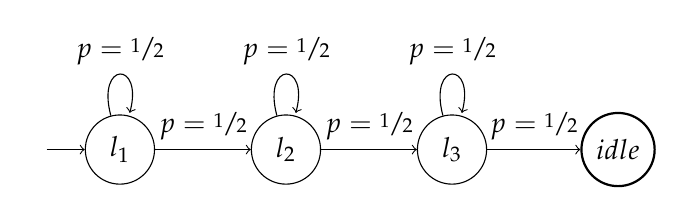
\begin{tikzpicture}[->,node distance=6em]
  \node[state] (l1) {$l_1$};
  \node (s) [xshift=-3em] {};
  \node[state] (l2) [right of=l1] {$l_2$};
  \node[state] (l3) [right of=l2] {$l_3$};
  \node[thick,state] (idle) [right of=l3] {$idle$};

  \path (s) edge node {} (l1)
        (l1) edge [loop above] node {$p=\sfrac{1}{2}$} (l1)
        (l1) edge node[above] {$p=\sfrac{1}{2}$} (l2)
        (l2) edge [loop above] node {$p=\sfrac{1}{2}$} (l2)
        (l2) edge node[above] {$p=\sfrac{1}{2}$} (l3)
        (l3) edge [loop above] node {$p=\sfrac{1}{2}$} (l3)
        (l3) edge node[above] {$p=\sfrac{1}{2}$} (idle);
\end{tikzpicture} \\[1ex]

In randomized scheduling, the weights of each element of the vector corresponds with random probabilities $p(i)$.

\begin{enumerate}
  \item Initialize $i$ with 1.
  \item If $v_i$ is not runnable, remain idle.
  \item With $p(i)$ probability, schedule $v_i$.
  \item Otherwise, increment $i$ and repeat from step 2.
\end{enumerate}

In round-robin scheduling, the weights of each element are used to divide time into arbitrarily many slices and schedule each of these with the frequency $p(i)$.

\begin{enumerate}
  \item Initialize $i$ with 1.
  \item If $v_i$ is not runnable, remain idle.
  \item If $i$ was skipped at the last scheduling decision for $i$, schedule $v_i$.
  \item Otherwise, skip it, increment $i$ and repeat from step 2.
\end{enumerate}

\subsection{Updating the scheduling vector}

The scheduling vector allows an arbitrary number of labels.  However, in order to achieve the same benefit as time donation discussed in Section \ref{s:donate}, the order of elements in the vector should be changed dynamically in a way that minimizes wasted time due to idleness while protecting against timing attacks.

When thread $t$ changes from Ready to Blocked,

\begin{itemize}
  \item swap schedule position of $t$ with thread $t'$ with $l_{t'} \sqsubseteq l_t$ and $t'$ is the last such thread.
\end{itemize}

When thread $t$ changes from Blocked to Ready or gets created,

\begin{itemize}
  \item if newly created, add $t$ add the end of $v$;
  \item swap schedule position of $t$ with thread $t'$ with $l_{t} \sqsubseteq l_{t'}$ and $t'$ is the first such thread.
\end{itemize}

When thread $t$ terminates,

\begin{itemize}
  \item if $t$ was last non-terminated thread at this level in the lattice, just remove it from $v$;
  \item otherwise, assign $t'$ to the slot of $t$ with $l_{t'} \sqsubseteq l_t$ and $t'$ is the last such thread.
\end{itemize}

% \begin{theorem}[Correctness (level)]
%   Evaluating a program in a security level $l$ as part of SME will result in the same observable behavior for channels labeled $l$ as running the program without SME if no channels above $l$ were opened.
% \begin{align*}
% \forall e,~ l.~~&\emptyset, e \rightarrow^{*}_l~C,v ~\wedge~\emptyset,e \rightarrow^{*} C',v'~\wedge  \\
%                 & \neg \exists {(l',\_,\_) \in C'} . l' > l ~\Rightarrow \\ & v' = v~\wedge~ ~\{ \vec{n} ~|~ (l, \_, \vec{n}) \in C' \} = \{ \vec{n} ~|~ (l, \_, \vec{n}) \in C \}
% \end{align*}
% \label{th:lvl}
% \end{theorem}

% \begin{theorem}[Correctness (all)]
%   Evaluating a program for all security levels program as part of SME will result in the same observable behavior as running the program without SME if .
% \begin{align*}
% \forall e,~ l.~~&\emptyset, e \rightarrow^{*}_L~C,v ~\wedge~\emptyset,e \rightarrow^{*} C',v' ~\Rightarrow \\ & v = v'~\wedge~ ~\{ \vec{n} ~|~ (l, \_, \vec{n}) \in C' \} = \{ \vec{n} ~|~ (l, \_, \vec{n}) \in C \}
% \end{align*}
% \label{th:all}
% \end{theorem}

% Theorem \ref{th:all} follows from Theorem \ref{th:lvl}.

% \subsection{Timing attacks}



\section{Related work}

It is actually possible to ensure timing-sensitive non-interference while still allowing branches on private values, as shown by Kashyap et. al.~\cite{kashyap2011}.  They recognized that a custom scheduler could schedule public/low threads in a way that these cannot learn anything about the potential execution of higher/private threads.  Different scheduling strategies correspond to different trade-offs between correctness/starvation and performance.  Non-comparable labels in a lattice ($l \not \sqsubseteq l'~\wedge~l \not \sqsupseteq l'$) further complicate scheduling as two non-comparable threads have to be hidden from each other.  Nevertheless, timing-sensitive non-interference is actually possible and subsumes termination-sensitive non-interference.

% \section{Evaluation}



\section{Conclusions}


\bibliographystyle{unsrtnat}
\bibliography{references}

\end{document}
